\documentclass[12pt]{article}
\usepackage[hidelinks]{hyperref}    
\usepackage[all]{hypcap}
\usepackage{amssymb}
\usepackage{amsmath}
\usepackage{graphicx}
\graphicspath{{../images/}}
\title{\textbf{Analisi Matematica\\Funzioni goniometriche}}
\date{04 Ottobre 2024}
\author{Andrea Malvezzi}
\begin{document}
\maketitle
\pagebreak
\tableofcontents
\pagebreak
\section{Circonferenza goniometrica}
La circonferenza goniometrica è una speciale circonferenza, rappresentata dalla seguente equazione:
\begin{equation}
    x^2 + y^2 = 1 \label{eq:circ_goniom}
\end{equation}
Tale circonferenza ha inoltre lunghezza pari a $2\pi$.
\begin{figure}[!htb]
    \centering
    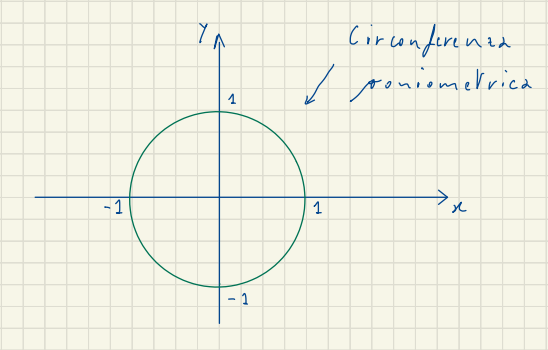
\includegraphics[width=1\textwidth, height=.7\textheight,keepaspectratio]{lezione_6/circonferenza_goniometrica.PNG}
    \begin{center}
        \caption{\label{fig:circ_goniom}La circonferenza goniometrica.}
    \end{center}
\end{figure}
\pagebreak
\subsection{Angoli in gradi e in radianti}
In questa circonferenza si opera basandosi su angoli, che possono essere espressi in \textit{gradi} oppure in \textit{radianti}.
\begin{figure}[!htb]
    \centering
    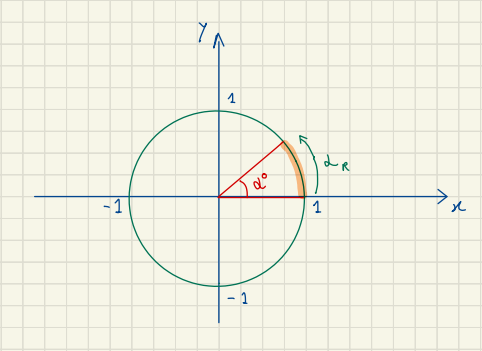
\includegraphics[width=1\textwidth, height=.7\textheight,keepaspectratio]{lezione_6/circonferenza_goniometrica_angolo.PNG}
    \begin{center}
        \caption{\label{fig:angolo_circonferenza}Un angolo $\alpha^{\circ}$ in gradi ed il suo corrispettivo in radianti $\alpha^r$.}
    \end{center}
\end{figure}\\
Per passare da un angolo in gradi ad uno in radianti, si usa la seguente proporzione:
\begin{equation}
    \alpha^{\circ}:360=\alpha^r:2\pi \label{eq:gradi_radianti}
\end{equation}
Che si può semplificare in:
\begin{equation}
    \alpha^r=\alpha^{\circ} \cdot \dfrac{\pi}{180}  \label{eq:gradi_radianti_solved}
\end{equation}
\section{Funzione Seno e Coseno}
Sia $P$ un punto sulla circonferenza goniometrica tale che $P(X_p,Y_p)$.\\
Allora:
\begin{equation}
    \begin{cases}
        P(X_p,Y_p),\\
        \sin{\alpha} = Y_p,\\
        \cos{\alpha} = X_p
        \label{eq:sin_cos_definizione}
    \end{cases}
\end{equation}
Che rappresentato sulla circonferenza goniometrica diventa:
\begin{figure}[!htb]
    \centering
    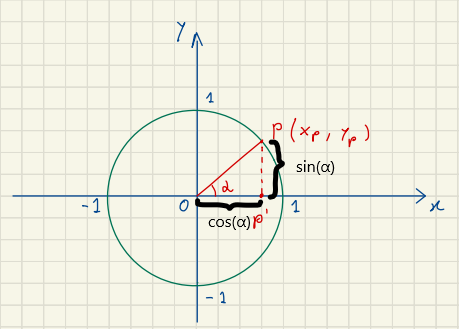
\includegraphics[width=1\textwidth, height=.7\textheight,keepaspectratio]{lezione_6/sin_cos_definizione.png}
    \begin{center}
        \caption{\label{fig:sin_cos_definizione}Il seno ed il coseno corrispondono ai due cateti di un triangolo rettangolo.}
    \end{center}
\end{figure}
\pagebreak
\subsection{Grafici}
In seguito i grafici della funzione seno e di quella coseno.
\begin{figure}[!htb]
    \centering
    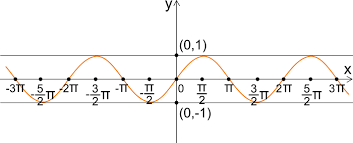
\includegraphics[width=1\textwidth, height=.7\textheight,keepaspectratio]{lezione_6/grafico_seno.png}
    \begin{center}
        \caption{\label{fig:grafico_seno}Grafico del seno.}
    \end{center}
\end{figure}
\begin{figure}[!htb]
    \centering
    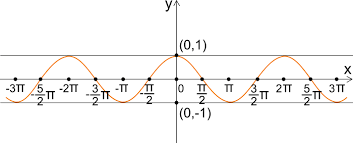
\includegraphics[width=1\textwidth, height=.7\textheight,keepaspectratio]{lezione_6/grafico_coseno.png}
    \begin{center}
        \caption{\label{fig:grafico_coseno}Grafico del coseno.}
    \end{center}
\end{figure}
\pagebreak
\subsection{Funzioni dispari e pari}
Inoltre, come facilmente osservabile dai grafici, invertendo il segno del parametro del coseno, si ottiene sempre lo stesso risultato, mentre invertendo quello del parametro del seno si ottiene un risultato a segno inverso.
Questo perché il coseno è una funzione \textbf{pari}, mentre il seno è \textbf{dispari}.
\begin{figure}[!htb]
    \centering
    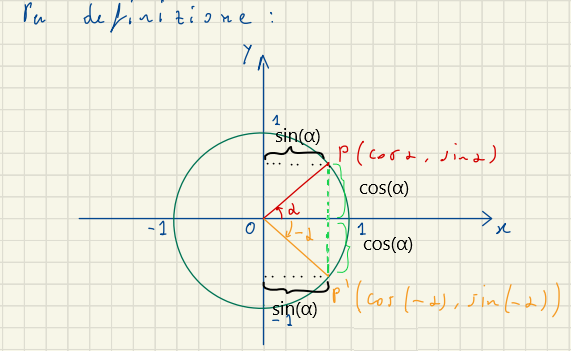
\includegraphics[width=1\textwidth, height=.7\textheight,keepaspectratio]{lezione_6/sin_cos_dispari_pari.PNG}
    \begin{center}
        \caption{\label{fig:sin_cos_dispari_pari}Esempio di parità del coseno e di disparità del seno.}
    \end{center}
\end{figure}
\section{Funzione Tangente}
La funzione tangente è definita secondo la seguente scrittura:
\begin{equation}
    \tan{\alpha} = \dfrac{\sin{\alpha}}{\cos{\alpha}}, \cos{\alpha} \not= 0 \label{eq:funzione_tangente}
\end{equation}
Inoltre, la tangente ha periodicità pari a $\pi$, e non a $2\pi$.
\subsection{Grafico della tangente}
A seguire il grafico della funzione tangente, con asintoto verticale in $\dfrac{\pi}{2} + k\pi$.
\begin{figure}[!htb]
    \centering
    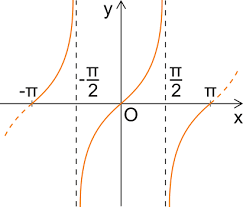
\includegraphics[width=1\textwidth, height=.7\textheight,keepaspectratio]{lezione_6/grafico_tangente.png}
    \begin{center}
        \caption{\label{fig:grafico_tangente}Grafico della tangente.}
    \end{center}
\end{figure}\\
\section{Tabella dei valori notevoli}
A seguire una tabella contenente alcuni valori notevoli delle funzioni goniometriche:
\begin{center}
    \begin{tabular}{|| c | c | c | c ||}
        \hline
        $\alpha$ (angolo) & $\sin{\alpha}$ & $\cos{\alpha}$ & $\tan{\alpha}$ \\
        \hline
        $0^{\circ}$ & $\sin{0} = 0$ & $\cos{0} = 1$ & $\tan{0} = 0$ \\
        \hline
        $30^{\circ} = \dfrac{\pi}{6}$ & $\sin{\dfrac{\pi}{6}} = \dfrac{1}{2}$ & $\cos{\dfrac{\pi}{6}} = \dfrac{\sqrt{3}}{2}$ & $\tan{\dfrac{\pi}{6}} = \dfrac{\sqrt{3}}{3}$ \\
        \hline
        $45^{\circ} = \dfrac{\pi}{4}$ & $\sin{\dfrac{\pi}{4}} = \dfrac{\sqrt{2}}{2}$ & $\cos{\dfrac{\pi}{4}} = \dfrac{\sqrt{2}}{2}$ & $\tan{\dfrac{\pi}{4}} = 1$ \\
        \hline
        $60^{\circ} = \dfrac{\pi}{3}$ & $\sin{\dfrac{\pi}{3}} = \dfrac{\sqrt{3}}{2}$ & $\cos{\dfrac{\pi}{3}} = \dfrac{1}{2}$ & $\tan{\dfrac{\pi}{3}} = \sqrt{3}$ \\
        \hline
        $90^{\circ} = \dfrac{\pi}{2}$ & $\sin{\dfrac{\pi}{2}} = 1$ & $\cos{\dfrac{\pi}{2}} = 0$ & $\tan{\dfrac{\pi}{2}} = \not\exists$ \\
        \hline
    \end{tabular}
\end{center}
\pagebreak
\section{Funzioni goniometriche e triangoli}
Le funzioni trigonometriche son quindi strettamente legate ai triangoli, specialmente quello rettangolo:
\begin{figure}[!htb]
    \centering
    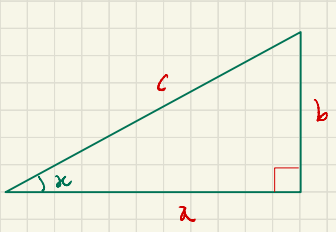
\includegraphics[width=1\textwidth, height=.7\textheight,keepaspectratio]{lezione_6/trigonometria.png}
    \begin{center}
        \caption{\label{fig:triangolo_rettangolo_trigonometria}In generale, per trovare uno dei vari lati di un triangolo rettangolo si moltiplica il seno o il coseno dell'angolo tra il lato in questione e l'ipotenusa.}
    \end{center}
\end{figure}\\
Dove:
\begin{itemize}
    \item \textit{a} = \textit{c} $\cdot \cos{\alpha}$
    \item \textit{b} = \textit{c} $\cdot \sin{\alpha}$
    \item \textit{c} = ipotenusa
    \item $\dfrac{b}{a} = \tan{\alpha} \rightarrow b = a \cdot \tan{\alpha}$
\end{itemize}
\section{Formule}
\subsection{Addizione e sottrazione}
Le formule di addizione e di sottrazione sono ideali per scrivere un'espressione in maniera semplificata, quando possibile.
\begin{equation}
    \cos({\alpha \pm \beta}) = \cos{\alpha} \cdot \cos{\beta} \mp \sin{\alpha} \cdot \cos{beta} \label{eq:somma_sottrazione_coseno}
\end{equation}
\begin{equation}
    \sin({\alpha \pm \beta}) = \sin{\alpha} \cdot \cos{\beta} \pm \cos{\alpha} \cdot \sin{\beta} \label{eq:somma_sottrazione_seno}
\end{equation}
\subsection{Duplicazione}
La formula di duplicazione è solamente un'estensione di quella di addizione, in quanto:
\begin{equation}
    \cos{2\alpha} = \cos({\alpha + \alpha}) = \cos^2{\alpha} - \sin^2{\alpha} = 
\end{equation}
\end{document}